\chapter{Clasificación con modelos multimodales (GPT-4o)}

En los últimos años, los grandes modelos de lenguaje multimodal han experimentado un crecimiento acelerado, tanto en capacidades como en su adopción en diversas áreas. Estos modelos tienen la habilidad de comprender, procesar y generar contenido integrando simultáneamente múltiples modalidades de datos, tales como texto, imágenes, audio, video y datos tabulares.

En particular, GPT-4o, el modelo multimodal más reciente desarrollado por OpenAI\footnote{GPT-4o lanzado el 13 de mayo de 2024. \url{https://openai.com/index/hello-gpt-4o/}}, es capaz de recibir entradas combinadas de texto e imágenes, y generar respuestas textuales coherentes y contextualizadas. Su diseño permite realizar tareas complejas mediante instrucciones en lenguaje natural, destacándose por su facilidad de uso, ya que está disponible mediante una interfaz de programación (API) que no requiere entrenamiento adicional específico por parte del usuario \parencites{openai2024gpt4o,shahriar2024gpt4o}. Estas características hacen que GPT-4o sea especialmente atractivo para aplicaciones prácticas en múltiples dominios donde se requiere una rápida adaptación y facilidad operativa, incluso por usuarios sin conocimientos técnicos profundos en aprendizaje automático.

El objetivo de esta sección es evaluar experimentalmente el rendimiento de dos estrategias de consulta a GPT-4o en comparación con nuestro modelo especializado (ResNet-18 fine-tuned). Aprovechando la facilidad de uso y la capacidad de generalización de los grandes modelos multimodales, basta con enviar cada imagen —o, en el segundo enfoque, pequeños ejemplos de referencia— al endpoint de OpenAI para obtener una predicción directa (“buena calidad” vs. “mala calidad”), sin necesidad de diseñar, entrenar o ajustar manualmente una red. De este modo, podemos medir qué precisión y utilidad práctica ofrece GPT-4o como alternativa de clasificación en el contexto del análisis automático de calidad de imágenes de fondo de ojo, y compararlo objetivamente con la solución basada en ResNet-18.

El proceso de consulta a GPT-4o se enmarca dentro del paradigma de \textit{in-context learning}, según el cual el modelo aprende a resolver una tarea a partir de la información (instrucciones y ejemplos) que se le proporciona directamente en el prompt, sin necesidad de un entrenamiento extenso o ajuste fino (fine-tuning) específico para cada tarea \parencites{chen2023gpt4vision}. De este modo, podemos distinguir dos modalidades principales:

\begin{itemize}
	\item \textbf{Zero-shot:} el modelo recibe únicamente una descripción de la tarea, sin ejemplos de referencia.
	\item \textbf{Few-shot:} además de la descripción, se incluyen unos pocos ejemplos etiquetados que sirven como contraste para guiar la predicción.
\end{itemize}

La muestra utilizada estuvo compuesta por 10.000 imágenes, con una proporción aproximada del 96\% correspondientes a imágenes de buena calidad (0) y 4\% de mala calidad (1), respetando la distribución real del conjunto de testeo.

\section{Zero-shot}
Se le presentó al modelo una imagen por vez, junto con un prompt en inglés que indicaba explícitamente la tarea:

\begin{table}[H]
	\renewcommand{\arraystretch}{3}
	\resizebox{\textwidth}{!}{
		\begin{tabular}{ ||l||  }
			\hline
			\makecell[l]{\textbf{Prompt:}\\
				\hspace*{3em}Classify the image as either 'Good quality' or 'Poor quality'. \\
				\hspace*{3em}Only respond with one of those two options.} \\
			\hline
		\end{tabular}
		}
	\caption{Prompt usado para clasificación zero-shot con GPT-4o.}
	\label{tab:promtZeroShot}
\end{table}

\begin{table}[H]
	\centering
	\renewcommand{\arraystretch}{1.5}
	\begin{tabular}{ ||ccccc||  }
		\hline
		\textbf{Clase} & \textbf{Precision} & \textbf{Recall} & \textbf{f1-score} & \textbf{Support} \\
		\hline
		0 (Buena) & 0.98 & 0.63 & 0.77 & 9,573 \\
		\hline
		1 (Mala) & 0.08 & 0.69 & 0.14 & 427 \\
		\hline
		Accuracy &  &  & 0.63 & 10,000 \\
		\hline
		Macro promedio & 0.53 & 0.66 & 0.45 & 10,000 \\
		\hline
		Promedio ponderado & 0.94 & 0.63 & 0.74 & 10,000 \\
		\hline
	\end{tabular}
	\caption{Classification report del modelo GPT-4o, modalidad zero-shot, evaluado sobre la muestra de test.}
	\label{tab:evaluacionZeroShot}
\end{table}

\begin{table}[H]
	\centering
	\renewcommand{\arraystretch}{1.5}
	\begin{tabular}{ ||lrr||  }
		\hline
		& \textbf{Predicho: Buena (0)} & \textbf{Predicho: Mala (1)} \\
		\hline
		Real: Buena (0) & 6,025 & 3,548 \\
		\hline
		Real: Mala (1) & 132  & 295 \\
		\hline
	\end{tabular}
	\caption{Matriz de confusión del modelo GPT-4o, modalidad zero-shot, evaluado sobre la muestra de test.}
	\label{tab:matrizZeroShot}
\end{table}

Se observa que, aunque el modelo logra identificar una parte significativa de las imágenes de mala calidad (recall 69\%), su precisión sobre esa clase es extremadamente baja (8\%), lo que indica una alta tasa de falsos positivos.

El F1-score para la clase 1 fue apenas 14\%, lo cual revela una clara dificultad del modelo en distinguir correctamente las imágenes de mala calidad en ausencia de contexto visual. En contraste, el desempeño sobre la clase mayoritaria (buena calidad) fue más equilibrado, con un F1-score de 77\%.

\subsection{Evaluación cualitativa con explicaciones generadas por GPT-4o modalidad zero shot}
Con el objetivo de analizar el razonamiento del modelo multimodal, se tomaron las tres imágenes (\ref{fig:gram1}, \ref{fig:gram2}, \ref{fig:gram3}) previamente utilizadas para generar mapas de activación Grad-CAM con la red ResNet-18 ajustada. Estas imágenes fueron procesadas individualmente por GPT-4o, esta vez utilizando un prompt extendido que solicitaba una predicción acompañada de una explicación detallada:

\begin{table}[H]
	\renewcommand{\arraystretch}{5}
	\resizebox{\textwidth}{!}{
		\begin{tabular}{ ||l||  }
			\hline
			\makecell[l]{\textbf{Prompt:}\\
				\hspace*{3em}Instruction: classify the image as either 'Good quality' or 'Poor quality'.\\
				\hspace*{3em}Please first output one line with the predicted label.\\
				\hspace*{3em}In the next line, provide a comprehensive explanation of your classification.\\
				\hspace*{3em}Consider image quality aspects such as sharpness, brightness, contrast, and the \\
				\hspace*{3em}visibility of anatomical structures like the optic disc, macula, and vessels.}\\
			\hline
		\end{tabular}
	}
	\caption{Prompt usado para clasificación zero-shot con GPT-4o.}
	\label{tab:promtZeroShotExplicacion}
\end{table}

A continuación, se presentan los resultado:

\begin{enumerate}
	\item \textbf{Imagen:} \ref{fig:gram1}:
	\begin{itemize}
		\item \textbf{Label real:} Mala calidad (1).
		\item \textbf{Predicción ResNet:} Mala calidad (1).
		\item \textbf{Predicción GPT-4o Zero-shot:} Good quality (0).
		\item \textbf{Explicación GPT-4o Zero-shot:} The image exhibits clear visibility of key anatomical structures such as the optic disc, macula, and blood vessels. The sharpness is adequate, with distinct and well-defined vessel outlines. The brightness and contrast levels are balanced, helping to highlight important details and ensuring that the overall view is not obscured by excessive dark or bright areas.
	\end{itemize}
	\item \textbf{Imagen:} \ref{fig:gram2}:
		\begin{itemize}
		\item \textbf{Label real:} Mala calidad (1).
		\item \textbf{Predicción ResNet:} Buena calidad (0).
		\item \textbf{Predicción GPT-4o Zero-shot:} Good quality (0).
		\item \textbf{Explicación GPT-4o Zero-shot:} The image is classified as 'Good quality' because it demonstrates clear visibility of essential anatomical structures such as the optic disc, macula, and vessels. The sharpness is sufficient, with distinct outlines of the retinal features. The brightness and contrast are well-balanced, providing a clear view of the different elements within the eye.
	\end{itemize}
	\item \textbf{Imagen:} \ref{fig:gram3}:
	\begin{itemize}
		\item \textbf{Label real:} Buena calidad (0).
		\item \textbf{Predicción ResNet:} Mala calidad (1).
		\item \textbf{Predicción GPT-4o Zero-shot:} Poor quality (1).
		\item \textbf{Explicación GPT-4o Zero-shot:} The image is classified as poor quality because it lacks sufficient brightness and sharpness, making it difficult to discern key anatomical structures such as the optic disc, macula, and blood vessels. The overall image is dark, and there is a lack of contrast, which further obscures important details necessary for a clear analysis.
	\end{itemize}
\end{enumerate}

En los tres casos analizados, el modelo GPT-4o en modalidad zero-shot demostró prestar atención a aspectos similares a los considerados por el modelo ResNet-18 ajustado, tales como la nitidez de las estructuras anatómicas, el contraste y la iluminación general de la imagen. Sin embargo, en el primer ejemplo, GPT-4o no logró identificar un artefacto crítico, un reflejo de la cámara, que determinaba la calidad de la imagen. Este defecto fue correctamente detectado por la red ResNet fine-tuned, lo que sugiere que, además de no estar específicamente entrenado en el dominio, el modelo puede verse limitado por la formulación del prompt. Es posible que la omisión de instrucciones explícitas sobre la detección de artefactos haya contribuido a esta predicción errónea, lo que refuerza la importancia del diseño del prompt al evaluar modelos multimodales en contextos clínicos. Esto motivó una segunda prueba, en la que se reformuló el prompt incluyendo de manera explícita la necesidad de considerar artefactos técnicos como reflejos y desenfoques.

\begin{table}[H]
	\renewcommand{\arraystretch}{5}
	\resizebox{\textwidth}{!}{
		\begin{tabular}{ ||l||  }
			\hline
			\makecell[l]{\textbf{Prompt:}\\
				\hspace*{3em}Instruction: classify the image as either 'Good quality' or 'Poor quality'.\\
				\hspace*{3em}Please first output one line with the predicted label.\\
				\hspace*{3em}In the next line, provide a comprehensive explanation of your classification.\\
				\hspace*{3em}Consider image quality aspects such as sharpness, brightness, contrast, and the \\
				\hspace*{3em}visibility of anatomical structures like the optic disc, macula, and vessels. \\
				\hspace*{3em}Also consider the presence of image artifacts such as glare, reflections, \\
				\hspace*{3em}vignetting, blurred edges, or any other technical issues that may impair diagnostic usability.}\\
			\hline
		\end{tabular}
	}
	\caption{Prompt usado para clasificación e interpretación zero-shot con GPT-4o, incluyendo en el prompt la necesidad de considerar artefactos.}
	\label{tab:promtZeroShotExplicacionArtefactos}
\end{table}

A continuación, se presentan los resultado:

\begin{enumerate}
	\item \textbf{Imagen:} \ref{fig:gram1}:
	\begin{itemize}
		\item \textbf{Label real:} Mala calidad (1).
		\item \textbf{Predicción ResNet:} Mala calidad (1).
		\item \textbf{Predicción GPT-4o Zero-shot:} Good quality (0).
		\item \textbf{Predicción GPT-4o Zero-shot (menciona artefactos en el prompt):} Poor quality (1).
		\item \textbf{Explicación GPT-4o Zero-shot (menciona artefactos en el prompt):} The image is classified as poor quality due to several factors: 
		1. \textbf{Sharpness}: The image appears blurry, and the details of anatomical structures like the optic disc and macula may not be clearly visible.
		2. \textbf{Brightness and Contrast}: The image seems to lack the proper balance of brightness and contrast, making it difficult to distinguish between different structures.
		3. \textbf{Artifacts}: There is a noticeable \textcolor{red}{glare at the center}, which could obscure important diagnostic features. Additionally, there is some vignetting around the edges, further diminishing image usability.
		4. \textbf{Visibility of Structures}: Given the blurriness and glare, it may be challenging to accurately assess the vessels and other critical areas for diagnostic purposes. Overall, these issues significantly impair the diagnostic usability of the image.
	\end{itemize}
	\item \textbf{Imagen:} \ref{fig:gram2}:
	\begin{itemize}
		\item \textbf{Label real:} Mala calidad (1).
		\item \textbf{Predicción ResNet:} Buena calidad (0).
		\item \textbf{Predicción GPT-4o Zero-shot:} Good quality (0).
		\item \textbf{Predicción GPT-4o Zero-shot (menciona artefactos en el prompt):} Poor quality (1).
		\item \textbf{Explicación GPT-4o Zero-shot (menciona artefactos en el prompt):} The image suffers from significant issues that impair its diagnostic usability. There is a prominent blurred area in the center, which obscures critical anatomical structures like the macula and part of the retinal vessels. Additionally, there is glare or reflections that further obscure the visibility. Although the optic disc is somewhat visible, the overall sharpness and contrast of the image are inadequate, with a lack of clarity and definition in the vessels and surrounding areas. These artifacts significantly impact the image quality, making it unsuitable for diagnostic purposes.
	\end{itemize}
	\item \textbf{Imagen:} \ref{fig:gram3}:
	\begin{itemize}
		\item \textbf{Label real:} Buena calidad (0).
		\item \textbf{Predicción ResNet:} Mala calidad (1).
		\item \textbf{Predicción GPT-4o Zero-shot:} Poor quality (1).
		\item \textbf{Predicción GPT-4o Zero-shot (menciona artefactos en el prompt):} Poor quality (1).
		\item \textbf{Explicación GPT-4o Zero-shot (menciona artefactos en el prompt):} The image appears to be of poor quality due to several factors. It's dark, lacking sufficient brightness and contrast to clearly distinguish anatomical structures like the optic disc, macula, and blood vessels. These key features are not clearly visible, which impacts its diagnostic usability. There are noticeable artifacts such as glare and blurred areas that further reduce the overall image quality. These issues collectively impair the clarity and diagnostic value of the retinal image.
	\end{itemize}
\end{enumerate}

Como resultado, GPT-4o no solo cambió sus predicciones, clasificando las tres imágenes como de mala calidad, sino que también ofreció explicaciones más detalladas en las que mencionó los artefactos detectados.

Sin embargo, este comportamiento plantea interrogantes. Por un lado, el modelo parece volverse más sensible a la presencia de cualquier elemento mencionado en el prompt, sin necesariamente evaluar si dicho defecto compromete efectivamente la utilidad clínica de la imagen. Por otro, se observa hasta qué punto la formulación del prompt condiciona el tipo de respuesta: lejos de ser una herramienta objetiva, GPT-4o adapta su criterio según las instrucciones, lo que implica un riesgo de sesgo si el diseño del prompt no está cuidadosamente calibrado. Por eso, aunque la capacidad del modelo para detectar artefactos mejora, es necesario comprobar si esas decisiones realmente ayudan al diagnóstico en la práctica. No alcanza con que el modelo diga algo razonable, hace falta validar que sus respuestas sean útiles y correctas en el contexto clínico donde se piensa aplicar.



\section{Few-shot}
En este caso, a diferencia del escenario zero-shot, se le presentaron al modelo tres imágenes de forma simultánea, combinadas en una sola figura. Las imágenes de referencia fueron extraídas del conjunto de entrenamiento, mientras la tercera imágen, sin etiqueta visible, corresponde al conjunto de test.

\begin{center}
	\begin{figure}[H]
		\centering
		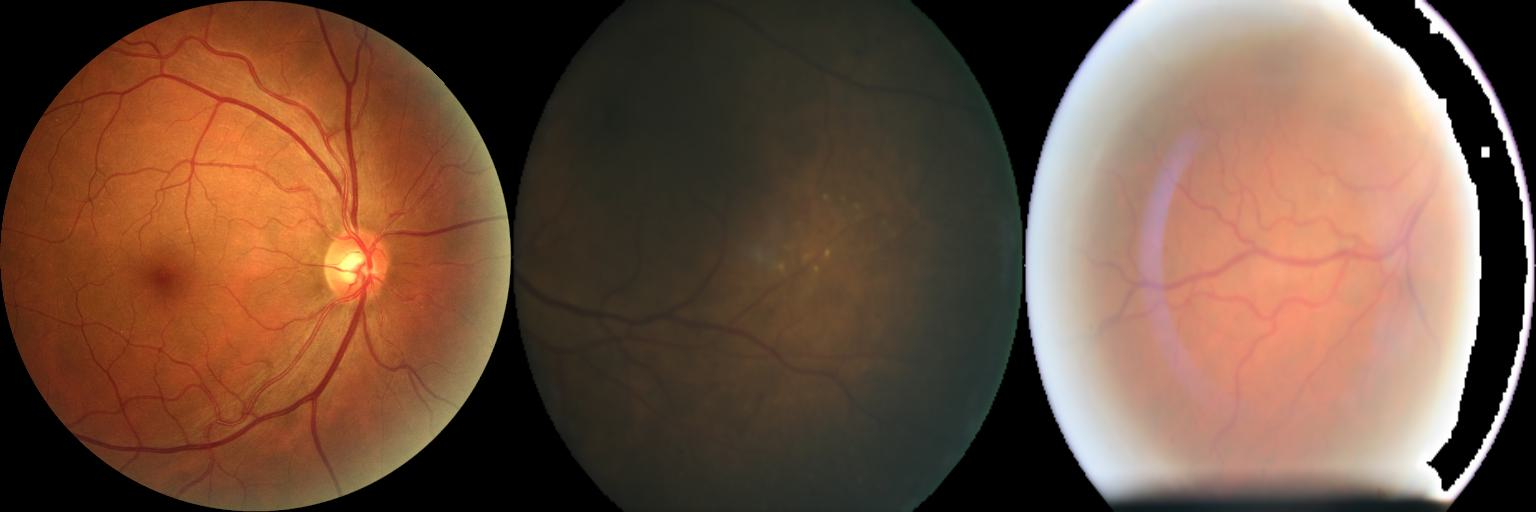
\includegraphics[scale=0.25]{doc_images/composite_test.jpg}
		\caption{Ejemplo de imagen compuesta utilizada en el esquema few-shot: buena calidad, mala calidad y muestra a clasificar (de izquierda a derecha).} 
		\label{fig:composite_test}
	\end{figure}
\end{center}

\begin{table}[H]
	\renewcommand{\arraystretch}{5}
	\resizebox{\textwidth}{!}{
		\begin{tabular}{ ||l||  }
			\hline
			\makecell[l]{\textbf{Prompt:}\\
				\hspace*{3em}Instruction: classify the images into two classes: 'Good quality', 'Poor quality'.\\
				\hspace*{3em}Example: the label of the above images:\\
				\hspace*{3em}Image 1: Good quality\\
				\hspace*{3em}Image 2: Poor quality\\
				\hspace*{3em}Please output one line with the predicted label for Image 3.}\\
			\hline
		\end{tabular}
	}
	\caption{Prompt usado para clasificación few-shot con GPT-4o.}
	\label{tab:promtFewShot}
\end{table}

Este diseño le permite al modelo inferir las características que definen cada clase a partir de ejemplos visuales, antes de emitir su predicción sobre la tercera imagen. Todas las imágenes de evaluación fueron clasificadas individualmente bajo esta modalidad, manteniendo constantes las dos imágenes de referencia (una buena y una mala) en todos los casos.

Dado que GPT-4o no conserva memoria entre solicitudes individuales, cada predicción se realiza de manera independiente, sin influencias del desbalance de clases presente en el conjunto evaluado. Esto implica que el modelo no ajusta su criterio de decisión en función de la frecuencia relativa de cada clase, como sí podría ocurrir en modelos entrenados explícitamente sobre el dominio.

\begin{table}[H]
	\centering
	\renewcommand{\arraystretch}{1.5}
	\begin{tabular}{ ||ccccc||  }
		\hline
		\textbf{Clase} & \textbf{Precision} & \textbf{Recall} & \textbf{f1-score} & \textbf{Support} \\
		\hline
		0 (Buena) & 0.98 & 0.51 & 0.67 & 9,573 \\
		\hline
		1 (Mala) & 0.07 & 0.78 & 0.12 & 427 \\
		\hline
		Accuracy &  &  & 0.52 & 10,000 \\
		\hline
		Macro promedio & 0.52 & 0.65 & 0.40 & 10,000 \\
		\hline
		Promedio ponderado & 0.94 & 0.52 & 0.65 & 10,000 \\
		\hline
	\end{tabular}
	\caption{Classification report del modelo GPT-4o, modalidad few-shot, evaluado sobre la muestra de test.}
	\label{tab:evaluacionFewShot}
\end{table}

\begin{table}[H]
	\centering
	\renewcommand{\arraystretch}{1.5}
	\begin{tabular}{ ||lrr||  }
		\hline
		& \textbf{Predicho: Buena (0)} & \textbf{Predicho: Mala (1)} \\
		\hline
		Real: Buena (0) & 4,895 & 4,678 \\
		\hline
		Real: Mala (1) & 93  & 334 \\
		\hline
	\end{tabular}
	\caption{Matriz de confusión del modelo GPT-4o, modalidad few-shot, evaluado sobre la muestra de test.}
	\label{tab:matrizFewShot}
\end{table}

A pesar de agregar más información visual al contexto, el desempeño general fue inferior al observado en la modalidad zero-shot, con un accuracy global de apenas 52\%. En particular, el modelo mostró una alta sensibilidad para la clase minoritaria (recall 78\% para imágenes de mala calidad), pero una muy baja precisión (7\%), lo que implica una gran cantidad de falsos positivos. El F1-score para la clase 1 fue de 12\%, confirmando la dificultad del modelo para distinguir de manera precisa las imágenes de baja calidad, incluso cuando se le ofrecen ejemplos visuales. Por otro lado, el rendimiento sobre la clase mayoritaria también se vio afectado: el recall descendió al 51\%, con un F1-score de 67\%.

\subsection{Evaluación cualitativa con explicaciones generadas por GPT-4o modalidad few-shot}
Repetimos el experimento realizado para la modalidad zero-shot sobre las tres imágenes (\ref{fig:gram1}, \ref{fig:gram2}, \ref{fig:gram3}) previamente utilizadas para generar mapas de activación Grad-CAM con la red ResNet-18 ajustada. Estas imágenes fueron procesadas individualmente por GPT-4o, esta vez utilizando un prompt extendido que solicitaba una predicción acompañada de una explicación detallada:

\begin{table}[H]
	\renewcommand{\arraystretch}{5}
	\resizebox{\textwidth}{!}{
		\begin{tabular}{ ||l||  }
			\hline
			\makecell[l]{\textbf{Prompt:}\\
				\hspace*{3em}Instruction: classify the images into two classes: 'Good quality', 'Poor quality'.\\
				\hspace*{3em}Example: the label of the above images:\\
				\hspace*{3em}Image 1: Good quality\\
				\hspace*{3em}Image 2: Poor quality \\
				\hspace*{3em}Please output one line with the predicted label for Image 3.\\
				\hspace*{3em}In the next line, provide a comprehensive explanation of your classification.\\
				\hspace*{3em}Consider image quality aspects such as sharpness, brightness, contrast, and the\\
				\hspace*{3em}visibility of anatomical structures like the optic disc, macula, and vessels.}\\
			\hline
		\end{tabular}
	}
	\caption{Prompt usado para clasificación e interpretación few-shot con GPT-4o.}
	\label{tab:promtFewShotExplicacion}
\end{table}

A continuación, se presentan los resultado:

\begin{enumerate}
	\item \textbf{Imagen:} \ref{fig:gram1}:
	\begin{itemize}
		\item \textbf{Label real:} Mala calidad (1).
		\item \textbf{Predicción ResNet:} Mala calidad (1).
		\item \textbf{Predicción GPT-4o Few-shot:} Poor quality (1).
		\item \textbf{Explicación GPT-4o Few-shot:} The third image exhibits characteristics of poor quality. It appears to have lower brightness and contrast compared to a good quality image. The anatomical structures such as the optic disc, macula, and blood vessels are not as clearly visible or well-defined. These features make it difficult to assess the image for medical or diagnostic purposes, categorizing it as poor quality.
	\end{itemize}
	\item \textbf{Imagen:} \ref{fig:gram2}:
	\begin{itemize}
		\item \textbf{Label real:} Mala calidad (1).
		\item \textbf{Predicción ResNet:} Buena calidad (0).
		\item \textbf{Predicción GPT-4o Few-shot:} Poor quality (1)).
		\item \textbf{Explicación GPT-4o Few-shot:} The image exhibits low brightness and contrast, making it difficult to clearly distinguish the anatomical structures like the optic disc, macula, and vessels. The sharpness is not sufficient to provide a clear and detailed view, which is crucial for a good quality classification.
	\end{itemize}
	\item \textbf{Imagen:} \ref{fig:gram3}:
	\begin{itemize}
		\item \textbf{Label real:} Buena calidad (0).
		\item \textbf{Predicción ResNet:} Mala calidad (1).
		\item \textbf{Predicción GPT-4o Few-shot:} Poor quality (1).
		\item \textbf{Explicación GPT-4o Few-shot:} The third image exhibits several signs of poor quality. It lacks adequate sharpness, making the anatomical structures like the optic disc, macula, and retinal vessels difficult to discern. Additionally, the brightness and contrast are insufficient, resulting in a dim and washed-out appearance that further obscures important details necessary for proper examination and analysis. This lack of clarity and definition categorizes it as poor quality.
	\end{itemize}
\end{enumerate}

En esta configuración, GPT-4o clasificó las tres imágenes como de mala calidad y las explicaciones ofrecidas por el modelo sugieren que, GPT-4o tiende a comparar directamente la imagen a clasificar con las imágenes de ejemplo provistas, en lugar de aplicar un criterio clínico general. Por ejemplo, se observa que menciona diferencias relativas en brillo o contraste respecto a la imagen de referencia de buena calidad, lo que sugiere una evaluación basada en comparación visual directa más que en estándares absolutos. Esto introduce nuevas variables que impactan en la predicción: la selección específica de las imágenes de ejemplo y la cantidad de ejemplos utilizados. A diferencia de los modelos entrenables, aquí no está claro cuánto peso tiene el contenido visual de las imágenes versus el texto del prompt. Esta falta de transparencia complica la interpretación del razonamiento del modelo y refuerza la necesidad de calibrar cuidadosamente tanto el prompt como la selección de ejemplos para evitar sesgos en la clasificación.

